\section{Проектирование модели платформы для интерактивного формирования
запросов к языковым и генеративным нейросетям}
\label{sec:designing}
\subsection{Целевая аудитория}
Целевой аудиторией системы являются пользователи-разработчики и художники, которые будут работать с ней на равных правах (единый уровень доступа). Платформа спроектирована с учётом их потребностей: с одной стороны, она предоставляет гибкие инструменты для тонкой ручной настройки запросов, ценимые разработчиками, с другой – наглядный и интуитивно понятный интерфейс, упрощающий работу с текстовым описанием для творческих специалистов. В следующих разделах будут подробно рассмотрены назначение системы, характеристики пользователей, требования, архитектура и используемые решения, обоснованные сформулированными техническими требованиями.

\subsection{Назначение системы}
Основное назначение разработанной системы – обеспечить пользователям возможность эффективно формировать и улучшать запросы (промпты) для различных нейросетевых моделей генерации текста и изображений.
Платформа предназначена для поддержки полного цикла работы с промптом: от начального наброска идеи до получения удовлетворительного чернового результата. Она предоставляет единое интерактивное пространство для проектирования промптов, позволяя объединить несколько функций, которые ранее требовали разрозненных инструментов.

С помощью данной системы пользователи могут создавать и редактировать текстовые описания запросов, итеративно их уточняя и детализируя. Интеллектуальные функции платформы позволяют автоматически дополнять введённый текст недостающими деталями и контекстом, что помогает менее опытным пользователям (например, художникам, не обладающим глубокими навыками работы с языковыми моделями) получить более богатые описания. Встроенный модуль оценки качества анализирует сформулированный запрос и выдает количественный показатель (в диапазоне 0–100), отражающий ориентировочное качество промпта. Это даёт возможность сразу увидеть, насколько хорошо запрос может быть воспринят нейросетью, и при необходимости внести правки до генерации результата. Кроме того, система обеспечивает преобразование формата запроса под требования конкретной целевой модели: например, адаптирует описание под синтаксис, предпочтительный для модели генерации изображений или, наоборот, для диалоговой языковой модели. Наконец, реализован режим предварительного просмотра (preview), позволяющий по нажатию кнопки отправить текущий промпт в тестовом режиме модели (локальной LLaMA или внешней Fusion Brain) и получить пример отклика – сгенерированный фрагмент текста либо эскиз изображения.

Таким образом, платформа выполняет роль песочницы для промптов: разработчики могут отладить запросы для своих AI-модулей, а художники – подобрать оптимальные описания для генерации иллюстраций. За счёт возможности быстро просматривать результат и оценку, существенно сокращается число итераций «вслепую». Пользователи могут корректировать промпт до тех пор, пока не будут удовлетворены оценкой и предпросмотром, и лишь затем использовать его на основной целевой модели (например, в продакшн-системе либо в стороннем сервисе генерации). В итоге применение платформы позволяет повысить качество конечного генерируемого контента – будь то текстовые ответы модели или создаваемые изображения – и сделать процесс разработки промптов более эффективным и предсказуемым.

\subsection{ Характеристика пользователей}
\begin{figure}[htbp]
    \centering
    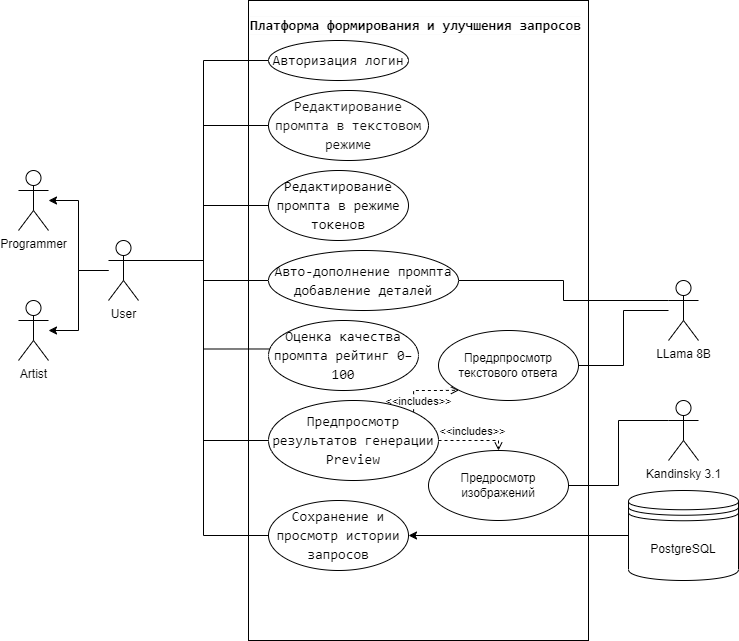
\includegraphics[width=0.8\textwidth]{picture/Диплом use case.png}
    \caption{Use case диаграмма платформы}
    \label{usecase}
\end{figure}
Как отмечалось, предполагаемые пользователи системы – это разработчики и художники, работающие с генеративными нейросетями. При проектировании платформы исходили из того, что эти две категории пользователей обладают разным опытом и целями, но обе нуждаются в удобном инструменте для создания хороших промптов. Уровень доступа в системе для них одинаковый (роль обычного пользователя), то есть все функции платформы доступны как разработчикам, так и представителям творческих профессий без каких-либо ограничений это можно заметить на диаграмме \ref{usecase}.

Разработчики (инженеры, специалисты по машинному обучению, авторы чат-ботов и др.) используют платформу преимущественно для отладки и улучшения текстовых запросов к языковым моделям. Для них важны гибкость и точность: они оценивают промпт с точки зрения логики обработки моделью, предсказывают, приведёт ли данная формулировка к нужному ответу. Разработчики, как правило, технически подкованы, поэтому им удобен режим прямого текстового редактирования промпта, возможность вручную корректировать даже мелкие детали формулировки. Они оценят также числовой показатель качества – метрику, которая поможет количественно сравнить разные варианты запросов. В их рабочем процессе платформа вписывается как инструмент быстрого прототипирования промптов: вместо того чтобы многократно вызывать целевую модель и получать от неё ответы для сравнения, разработчик может в интерактивном режиме довести один запрос до оптимального состояния, глядя на предварительные ответы от тестовой модели (LLaMA 8B) и на рейтинг качества. Получив удовлетворяющий результат, он переносит этот промпт в своё основное приложение или сервис.

Художники и специалисты по визуальному контенту (например, иллюстраторы, дизайнеры, концепт-художники) используют систему в несколько ином ключе – для создания описаний, на основе которых модели типа Stable Diffusion или Kandinsky генерируют изображения. Их цель – добиться, чтобы сформулированный текст точно передавал задуманный визуальный образ и стиль. Многие художники не имеют глубоких технических знаний, поэтому для них критична простота и наглядность интерфейса. Платформа учитывает это, предоставляя интуитивно понятные средства: режим редактирования через перетаскивание токенов особенно полезен, так как позволяет им воспринимать промпт не как сплошной текст, а как набор отдельных элементов или слов, из которых складывается описание сцены. Перемещая эти элементы, художник может экспериментировать с композицией фразы, не задумываясь о синтаксисе – система автоматически обновит текст запроса. Функция автоматического дополнения детализацией полезна для художника тем, что нейросеть сама предложит дополнительные детали (например, обстановку, освещение, стилистические прилагательные), которые могут улучшить итоговое изображение. Предпросмотр через API Fusion Brain позволяет им практически мгновенно увидеть черновой результат: например, эскиз сгенерированного изображения по текущему описанию. Это визуальная обратная связь чрезвычайно ценна – художник сразу поймёт, в правильном ли направлении двигается, и при необходимости скорректирует промпт (добавит или уберёт детали, изменит формулировку).

Важно подчеркнуть, что система не вводит разграничений между разработчиками и художниками на уровне функционала. И те, и другие работают в одной среде с идентичными возможностями. Это решение принято исходя из многопрофильности современных команд: нередко разработчики и дизайнеры работают совместно над проектами с AI, и им удобно использовать единый инструмент. Платформа удовлетворяет потребности обоих типов пользователей: обеспечивает достаточно тонкий контроль для удовлетворения запросов разработчиков и одновременно остается дружественной для творческих специалистов, не требуя от них знаний программирования. Такой подход расширяет потенциальную аудиторию системы и повышает её ценность в междисциплинарных командах.

\subsection{Технические требования}

Разработка платформы базируется на предварительно сформулированных технических требованиях, отражающих необходимый функционал и ограничения системы. Требования охватывают как функциональные возможности, видимые пользователю, так и нефункциональные характеристики (производительность, совместимость, безопасность и др.). Ниже перечислены ключевые требования к системе.

Функциональные требования (основной пользовательский функционал платформы):

\begin{enumerate}[label=\arabic*.]
    \item Редактирование запросов в текстовом и графическом режиме. Система должна предоставлять интерфейс для ввода и правки текста промпта вручную (классическое текстовое поле) и альтернативный интерфейс в виде списка токенов, которые пользователь может перемещать, удалять или заменять. Любое изменение последовательности токенов в графическом режиме должно незамедлительно отражаться в текстовом представлении промпта, и наоборот, обеспечивая двунаправленную синхронизацию. Должна поддерживаться работа с промптом произвольной длины (в разумных пределах, например до 1000 символов) и с различными символами, включая буквы разных алфавитов, цифры, знаки препинания и эмодзи (это важно, так как некоторые модели допускают использование эмодзи в описании изображения)\cite{fusionbrain:docs}. Пользователь должен видеть текст своего запроса и иметь возможность редактировать его удобным для себя способом.
    \item Автоматизированное дополнение (расширение) запроса деталями. Платформа должна по запросу пользователя уметь генерировать расширенную версию введённого промпта, добавляя к нему недостающую детализацию. Фактически, это интеллектуальный помощник: на основе исходного чернового текста запроса система (с помощью внутренней языковой модели) предлагает дополнительные описательные фразы, контекст или уточнения, которые могут сделать запрос более понятным для нейросети. Например, пользователь ввёл краткий запрос «кот сидит на дереве», а система может предложить дополнить: «кот сидит на дереве в лучах заходящего солнца, вокруг осенний пейзаж». Метод вызова – нажатие специальной кнопки («Дополнить»), после чего текущий текст промпта вместе с уже введёнными деталями остается, а к нему в конец или по соответствующим местам добавляется сгенерированный моделью текст (пользователь затем может отредактировать результат по своему усмотрению). Требуется, чтобы дополнение работало корректно для разных типов запросов (как описательных, так и вопросительных) и на двух основных языках (русский и английский), учитывая, что целевые модели поддерживают многоязычные запросы.
    \item Оценка качества промпта. В системе реализуется автоматическая оценка составленного пользователем запроса по шкале от 0 до 100. Эта оценка носит рекомендательный характер и должна отражать степень соответствия промпта лучшим практикам и ожидаемым требованиям модели. Пользователю отображается числовое значение или графический индикатор (например, цветовая индикация: красный – низкое качество, зелёный – высокое). Внутренне оценка может основываться на наборе правил или модели, анализирующих текст: учитывается длина запроса, специфичность формулировок, наличие деталей, отсутствие противоречий или запретов. Например, слишком короткий или расплывчатый запрос получит низкую оценку, а конкретный, содержательный запрос – более высокую. Чем более точно и понятно сформулирован промпт, тем выше должен быть рейтинг. (Это соответствует рекомендациям по промптингу: качество результатов зависит от того, сколько информации предоставлено и насколько хорошо запрос составлен)\cite{promptingguide:basics}. Данный модуль служит подсказкой: он должен быстро (в течение долей секунды) пересчитывать оценку при изменении текста и тем самым стимулировать пользователя улучшать запрос до получения приемлемого балла.
    \item Предварительный просмотр результата (preview). Одним из важнейших требований является возможность быстрой генерации чернового результата по текущему запросу. Пользователь, не покидая интерфейс редактора промптов, должен получить от системы пример отклика целевой модели – сгенерированный текст или изображение, соответствующее введённому описанию. Данный функционал реализуется двумя способами: для текстовых моделей – через локальную LLaMA 8B, для изображений – через вызов внешнего API Fusion Brain. Платформа должна определить, какой тип результата требуется (например, по выбранному целевому движку или по контексту: если пользователь редактирует текстовый запрос для чат-бота, то генерируется текст-ответ; если промпт адресован модели изображения, то генерируется картинка). После нажатия кнопки «Preview» происходит обращение к соответствующей модели:
    \begin{enumerate}[label=4.\arabic*.]
        \item В случае текста: LLaMA 8B генерирует продолжение или ответ на заданный промпт (необходимо ограничить размер выдаваемого фрагмента, например 1000 символов, чтобы получить быстрый предварительный ответ). Полученный ответ отображается на экране (например, в отдельном поле под запросом).
        \item В случае изображения: сервер отправляет запрос к API Fusion Brain (модель Kandinsky 3.1) с параметрами генерации (тип = GENERATE, текст запроса и др.). В ответ через некоторое время возвращается сгенерированное изображение, которое выводится пользователю (в виде эскиза, уменьшенного изображения либо полноразмерного, если позволяет интерфейс). Пользователь должен иметь возможность быстро увидеть этот результат в интерфейсе, без ручного перехода на внешние сервисы. Например, платформа может отобразить сгенерированную картинку прямо в браузере. В обоих случаях предварительно сгенерированный контент носит ознакомительный характер – он позволяет оценить, что примерно получится из данного промпта. Пользователь, проанализировав результат, может тут же подправить запрос и снова вызвать preview, добиваясь улучшения. Важно, чтобы среднее время получения предпросмотра было приемлемым: для текста это обычно менее 5 секунд, для изображения – порядка 5–15 секунд (зависит от мощности сервера и скорости внешнего API).
    \end{enumerate}
\end{enumerate}
Помимо основных функций, вытекают и общие технические требования к системе: 
\begin{enumerate}[label=\arabic*.]
    \item Интуитивность и удобство интерфейса. Пользователи разных категорий должны легко освоить работу с платформой. Интерфейс должен быть локализован (минимум на русском языке, так как аудитория – в том числе русскоговорящие художники). Все элементы (кнопки «Оценить», «Предпросмотр», переключатель режима редактирования и т.д.) должны быть наглядно обозначены. Требуется реализация динамического обновления – например, пересчёт оценки качества без перезагрузки страницы, мгновенная синхронизация текстового и токенного представления запроса. Это подразумевает использование возможностей SPA (Vue.js) для реактивности.
    \item  Производительность и масштабируемость. Платформа должна эффективно работать при одновременном использовании несколькими пользователями. Ожидается, что число активных пользователей невелико (например, единицы или десятки, поскольку целевая аудитория – команда разработчиков или художников или отдельные специалисты), однако архитектура не должна иметь жёстких ограничений на масштабирование. Серверная часть на FastAPI должна обрабатывать параллельно несколько запросов (благодаря асинхронности и производительности FastAPI это достижимо)\cite{fastapi:practicum}. Важно оптимизировать время отклика: интерактивные операции (редактирование, оценка) происходят почти мгновенно, а более тяжёлые (предпросмотр) – максимально быстро для выбранных моделей. Для ускорения генерации текста модель LLaMA загружается в память заранее и остаётся в режиме ожидания запросов, чтобы не тратить время на инициализацию при каждом preview. Для Fusion Brain API можно предусмотреть обработку в асинхронном режиме (не блокируя основной поток приложения во время ожидания ответа от внешнего сервиса).
    \item Ограничения и обработка ошибок. Система должна корректно обрабатывать нестандартные ситуации: слишком длинные запросы (превышающие лимиты модели) – выдавая предупреждение или автоматически укорачивая до допустимого размера; недопустимые символы – экранируя или удаляя их; отсутствие связи с внешним API – уведомляя пользователя о невозможности получить preview в данный момент. Все входные данные валидируются (FastAPI и Pydantic обеспечивают автоматическую проверку типов и форматов на уровне API\cite{yandex:fastapi}), а при обнаружении некорректных – сервер возвращает понятные сообщения об ошибках. Важным требованием является устойчивость: сбой одной из компонентов (например, недоступность БД или падение модели) не должен приводить к неуправляемому краху всего приложения – должны быть предусмотрены механизмы возврата в консистентное состояние или перезапуска сервиса.
    \item Совместимость и развиваемость. Платформа должна быть построена с использованием стандартных веб-технологий, обеспечивающих её совместимость с основными браузерами (Chrome, Firefox, Safari, Edge) без необходимости установки специальных плагинов. Желательно соблюдение принципов адаптивности интерфейса (возможность работать на экране ноутбука, настольного ПК, и, по возможности, на планшете). В архитектуре и коде должны быть заложены возможности расширения: например, добавление новых моделей (если в будущем понадобится поддержать другую нейросеть для генерации аудио или видео, или добавить ещё одну языковую модель) не должно требовать переписывания системы с нуля. Это означает, что компоненты (модуль оценки, модуль реструктуризации) должны быть реализованы конфигурируемо, с возможностью подключения новых правил или алгоритмов.
\end{enumerate}
Сформулированные выше требования служат основой для проектирования системы. На их основании в следующих разделах выбираются соответствующие методики и технические решения, обосновывается архитектура, алгоритмы работы и необходимые ресурсы. Соблюдение этих требований должно обеспечить, что итоговая платформа будет полнофункциональной, удобной для целевых пользователей и надёжной в эксплуатации.
\subsection{Архитектура системы}
\begin{figure}[htbp]
    \centering
    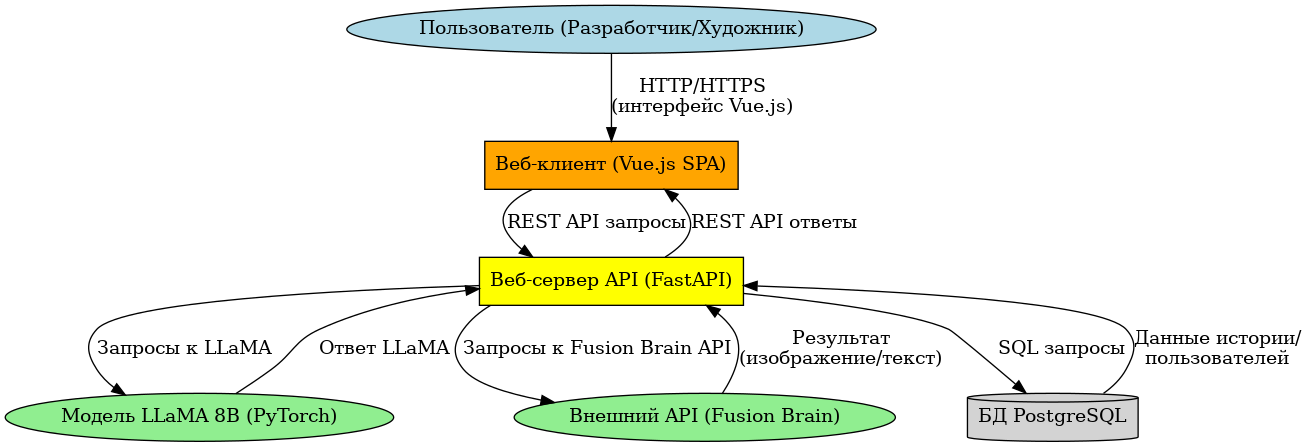
\includegraphics[width=0.8\textwidth]{picture/diploma-architecture.png}
    \caption{Архитектура платформы}
    \label{architecture}
\end{figure}
 Платформа имеет распределённую архитектуру типа «клиент–сервер». Это означает, что функциональность разделена между фронтендом (клиентским приложением, выполняющимся в браузере пользователя) и бекендом (серверным приложением, выполняющим бизнес-логику, взаимодействие с моделями и БД). На рисунке \ref{architecture} представлена структурная схема архитектуры системы с основными компонентами и потоками данных между ними.

Как показано на схеме, центральным звеном является веб-сервер API, реализованный на FastAPI. Этот сервер принимает входящие запросы от клиентского приложения по протоколу HTTP(S) и отвечает на них. Взаимодействие клиента и сервера происходит по REST API: для каждой функции предусмотрен соответствующий эндпойнт. Например, могут быть маршруты complete prompt (для дополнения детализации), valuate prompt (для оценки), transform prompt (для реструктуризации) и preview (для получения результата генерации). Клиентское приложение обращается к этим конечным точкам, передавая необходимые данные (тексты промптов, параметры) в формате JSON, и получает от сервера ответы, также закодированные в JSON (кроме случаев, когда передаются двоичные данные изображения). Обмен происходит по сети, предпочтительно с использованием шифрования (HTTPS) для безопасности.

Клиентская часть (Vue.js SPA) – это одностраничное приложение, загружаемое в браузер. Оно отвечает за отображение UI и интерактивность. После загрузки (HTML, CSS, JS) клиент устанавливает связь с сервером через AJAX-запросы (например, с помощью fetch API или библиотеки axios) к REST API. Вся логика по обновлению интерфейса – на стороне клиента: перемещение токенов, обновление текста, визуализация оценки (например, индикатор качества) – выполняется средствами JavaScript внутри браузера. Vue.js, являясь реактивным фреймворком, упрощает реализацию динамических компонентов интерфейса\cite{vuejs:wiki}. Например, текстовое поле и список токенов могут быть связанными реактивными данными: изменение одного автоматически отражается в другом. Клиент также обрабатывает элементы управления – кнопка «Оценить» может просто вызывать соответствующую функцию JS, которая отправит запрос на сервер и по получении ответа обновит отображаемую оценку. Аналогично, нажатие «Preview» инициирует последовательность: показать индикатор загрузки, отправить промпт на сервер, дождаться ответа и затем либо отобразить сгенерированный текст, либо встроить полученное изображение (например, через создание HTML-элемента <img> с полученными данными). Таким образом, фронтенд выполняет роль презентационного слоя, обеспечивая удобство для пользователя и минимизируя задержки взаимодействия (многие операции, не требующие ресурсов сервера, происходят мгновенно за счёт реактивности Vue).

Серверная часть (FastAPI) – сердце бизнес-логики платформы. FastAPI выбран благодаря его современной архитектуре, оптимизированной под высоконагруженные API и удобство разработки. Приложение FastAPI запускается, как правило, под управлением ASGI-сервера (например, Uvicorn), способного обрабатывать асинхронные запросы. Основные компоненты на стороне сервера:
\begin{enumerate}[label=\arabic*.]
    \item Контроллеры (роуты) API. В FastAPI разработаны обработчики для каждого метода API. Они принимают входные данные (автоматически распарсенные из JSON благодаря Pydantic-моделям), выполняют требуемые действия (например, вызывают модель или делают запрос к БД) и формируют ответ. Каждый такой контроллер работает по принципу: получить запрос -> вызвать соответствующую внутреннюю функцию или метод -> вернуть результат пользователю. Например, контроллер evaluate prompt получив JSON с полем prompt: "текст запроса", передаст эту строку в модуль оценки качества и вернёт клиенту JSON с полем score: 78 (пример).
    \item Модуль интеграции с LLaMA. Поскольку модель LLaMA 8B развёрнута локально, серверное приложение должно загружать и хранить эту модель в памяти, а также иметь методы для генерации текста. При запуске сервера происходит инициализация: с помощью библиотеки PyTorch и соответствующих средств (например, Hugging Face Transformers) модель загружается из файла весов. Благодаря интеграции напрямую в приложение, это называется встроенным (embedded) подходом – модель включена в состав сервиса и доступна как объект в коде\cite{}. Например, может быть создан singleton-объект llama model, который потом используется различными ручками API. Модель, находящаяся в оперативной памяти на GPU, может обрабатываться быстрыми вызовами – это значительно ускоряет получение ответа (не требуется каждый раз поднимать отдельный процесс или обращаться к удалённому API). Взаимодействие с LLaMA происходит через вызовы функций генерации: сервер формирует на основе пользовательского промпта вход для модели и вызывает метод model.generate() (либо аналогичный, в зависимости от используемой библиотеки), получая результат – сгенерированный текст. Этот текст затем отфильтровывается или обрабатывается по необходимости (например, обрезается до нужной длины) и пересылается клиенту.
    \item Модуль интеграции с Fusion Brain API. В случаях, когда требуется сгенерировать изображение, сервер выполняет роль клиента к внешнему API. Он делает HTTP-запрос (например, POST) к службе Fusion Brain, включая в него текст промпта и необходимые параметры (версия модели, желаемое разрешение изображения и т.д.). В ответ Fusion Brain возвращает данные изображения. Согласно документации, Kandinsky 3.1 позволяет получать изображения размером до 1024×1024; для предпросмотра сервер может запрашивать, к примеру, изображение 512×512 пикселей, чтобы сократить время ответа\cite{fusionbrain:docs}. Полученное изображение может приходить закодированным (например, URL ссылки на изображение или бинарные данные). Сервер, получив результат, преобразует его в формат, пригодный для пересылки фронтенду. Наиболее прямолинейный способ – переслать изображение как набор байт (в base64) или как ссылку, проксируемую через сервер. В реализации платформы может использоваться проксирование: сервер сохраняет картинку во временном хранилище (или просто держит в памяти) и отдаёт фронту по тому же API (например, ответ на preview для изображения содержит URL вида media preview123.png или непосредственный Base64). Клиентская часть затем отображает картинку пользователю. Взаимодействие с внешним API должно быть безопасным: ключ API Fusion Brain хранится на сервере (в конфигурации), и ни при каком условии не отправляется на клиент. Запросы должны выполняться с учётом возможных задержек (лучше асинхронно, чтобы не блокировать другие процессы сервера).
    \item Модуль работы с базой данных. Серверное приложение взаимодействует с PostgreSQL для хранения постоянных данных. Это включает регистрацию/авторизацию пользователей (см. раздел 9 о безопасности) и сохранение истории запросов. История запросов может храниться в виде таблицы: пользователь, текст промпта, время, возможно оценка и предпросмотр (например, ссылка на сохранённый результат). Обращения к базе данных реализованы через ORM (например, SQLAlchemy) либо через драйвер asyncpg для асинхронной работы. Использование ORM обеспечивает защиту от SQL-инъекций и удобство разработки – запросы к базе генерируются автоматически, что повышает надёжность хранения данных\cite{postgresql:skillfactory}, \cite{postgresql:wiki}. PostgreSQL, будучи одной из наиболее развитых свободных СУБД, гарантирует целостность данных и поддерживает все необходимые функции (ACID-транзакции, индексацию и пр.), что важно для ведения истории запросов без потерь. 
\end{enumerate}
Взаимодействие компонентов. Все компоненты связаны через чётко определённые интерфейсы. Браузерный клиент обращается к серверу только через API (не напрямую к БД или моделям). Сервер, в свою очередь, взаимодействует с LLaMA через вызовы функций (в памяти процесса) и с Fusion Brain через HTTP, а с базой – через SQL-запросы. Подобная модульность облегчает замену частей: например, можно обновить версию модели LLaMA или переключиться на другую языковую модель, не затрагивая логику фронтенда; либо заменить Fusion Brain на иной API генерации изображений, скорректировав лишь соответствующий модуль.

Архитектура поддерживает масштабирование: при возросшей нагрузке фронтенд-приложение может быть вынесено на отдельный CDN, а серверная часть – развёрнута в виде нескольких экземпляров за балансировщиком нагрузки. База данных может быть отдельно вынесена на кластер PostgreSQL для обеспечения высокой доступности. Так как сервер Stateless (не хранит сессии в памяти, вся важная информация – в БД), то масштабировать его горизонтально несложно. Единственный ограничивающий фактор – модель LLaMA, которая потребляет значительный объем GPU-ресурсов, поэтому в случае интенсивной нагрузки возможно использование нескольких серверов с каждой загруженной моделью (или альтернатива – вынесение модели в отдельный сервис). Но в расчёте на целевое применение (ограниченное число пользователей) текущая архитектура (один бекенд-инстанс с моделью) считается достаточной и оптимальной по простоте.

\subsection{Алгоритмическое и программное обеспечение}
В данном разделе описаны ключевые алгоритмы, реализующие функции платформы, а также используемое программное обеспечение (библиотеки, фреймворки) и принятые при разработке технические решения. Проектирование алгоритмов велось на основе требований, сформулированных в разделе 3.4, – каждый функциональный пункт соответствует определённой методике реализации. Также рассматриваются программные средства, обеспечивающие выполнение этих алгоритмов.

\begin{figure}[htbp]
    \centering
    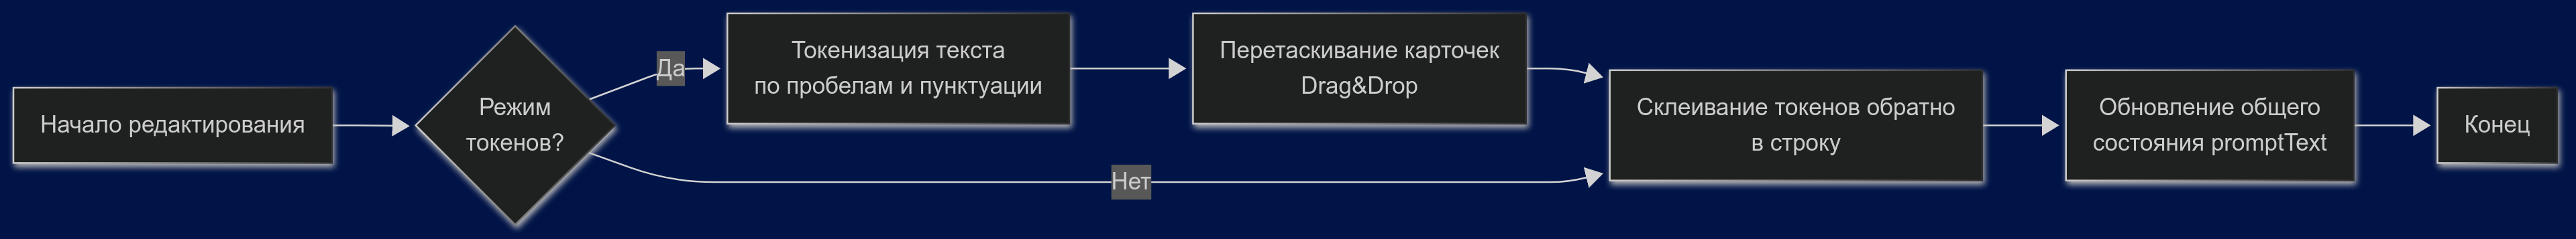
\includegraphics[width=1\textwidth]{picture/diploma-inter-algo-1.png}
    \caption{Алгоритм редактирования запроса}
    \label{algo-1}
\end{figure}

Редактирование запросов (текст и токены). Алгоритм редактирования в текстовом режиме тривиален и отображён на диаграмме \ref{algo-1}: пользователь вводит или изменяет строку символов, которая хранится во внутреннем состоянии приложения. Более интересен алгоритм представления промпта в виде набора токенов. Здесь под токеном понимается либо отдельное слово, либо устойчивое словосочетание – на практике для упрощения можно принять токенизацию по пробелам и знакам пунктуации (каждое слово или знак рассматривается как отдельный элемент). При переключении в режим токенов исходный текст промпта разбивается на массив токенов. Этот массив отображается на экране, например, в виде последовательности интерактивных «карточек» с текстом. Для реализации перетаскивания (drag-and-drop) используются возможности HTML5 DnD или готовые компоненты из экосистемы Vue (например, Vue.Draggable). Далее массив конкатенируется обратно в строку с добавлением пробелов – таким образом получается обновлённый текст промпта. Vue.js автоматически отследит изменение массива токенов и обновит связанную переменную текста (или наоборот, если связность сделана через одно хранилище состояния). Таким образом обеспечивается одновременная актуализация обоих представлений. Кроме того, если пользователь в текстовом поле ручным образом изменяет текст (например, дописывает новое слово), алгоритм распознаёт это (через реактивный watcher) и пересобирает список токенов заново. В результате редактирование может происходить параллельно в любом формате без рассинхронизации. Этот алгоритм достаточно прост (основные операции – разбиение строки и объединение списка), поэтому не нагружает систему даже при длинных промптах.
\begin{figure}[htbp]
    \centering
    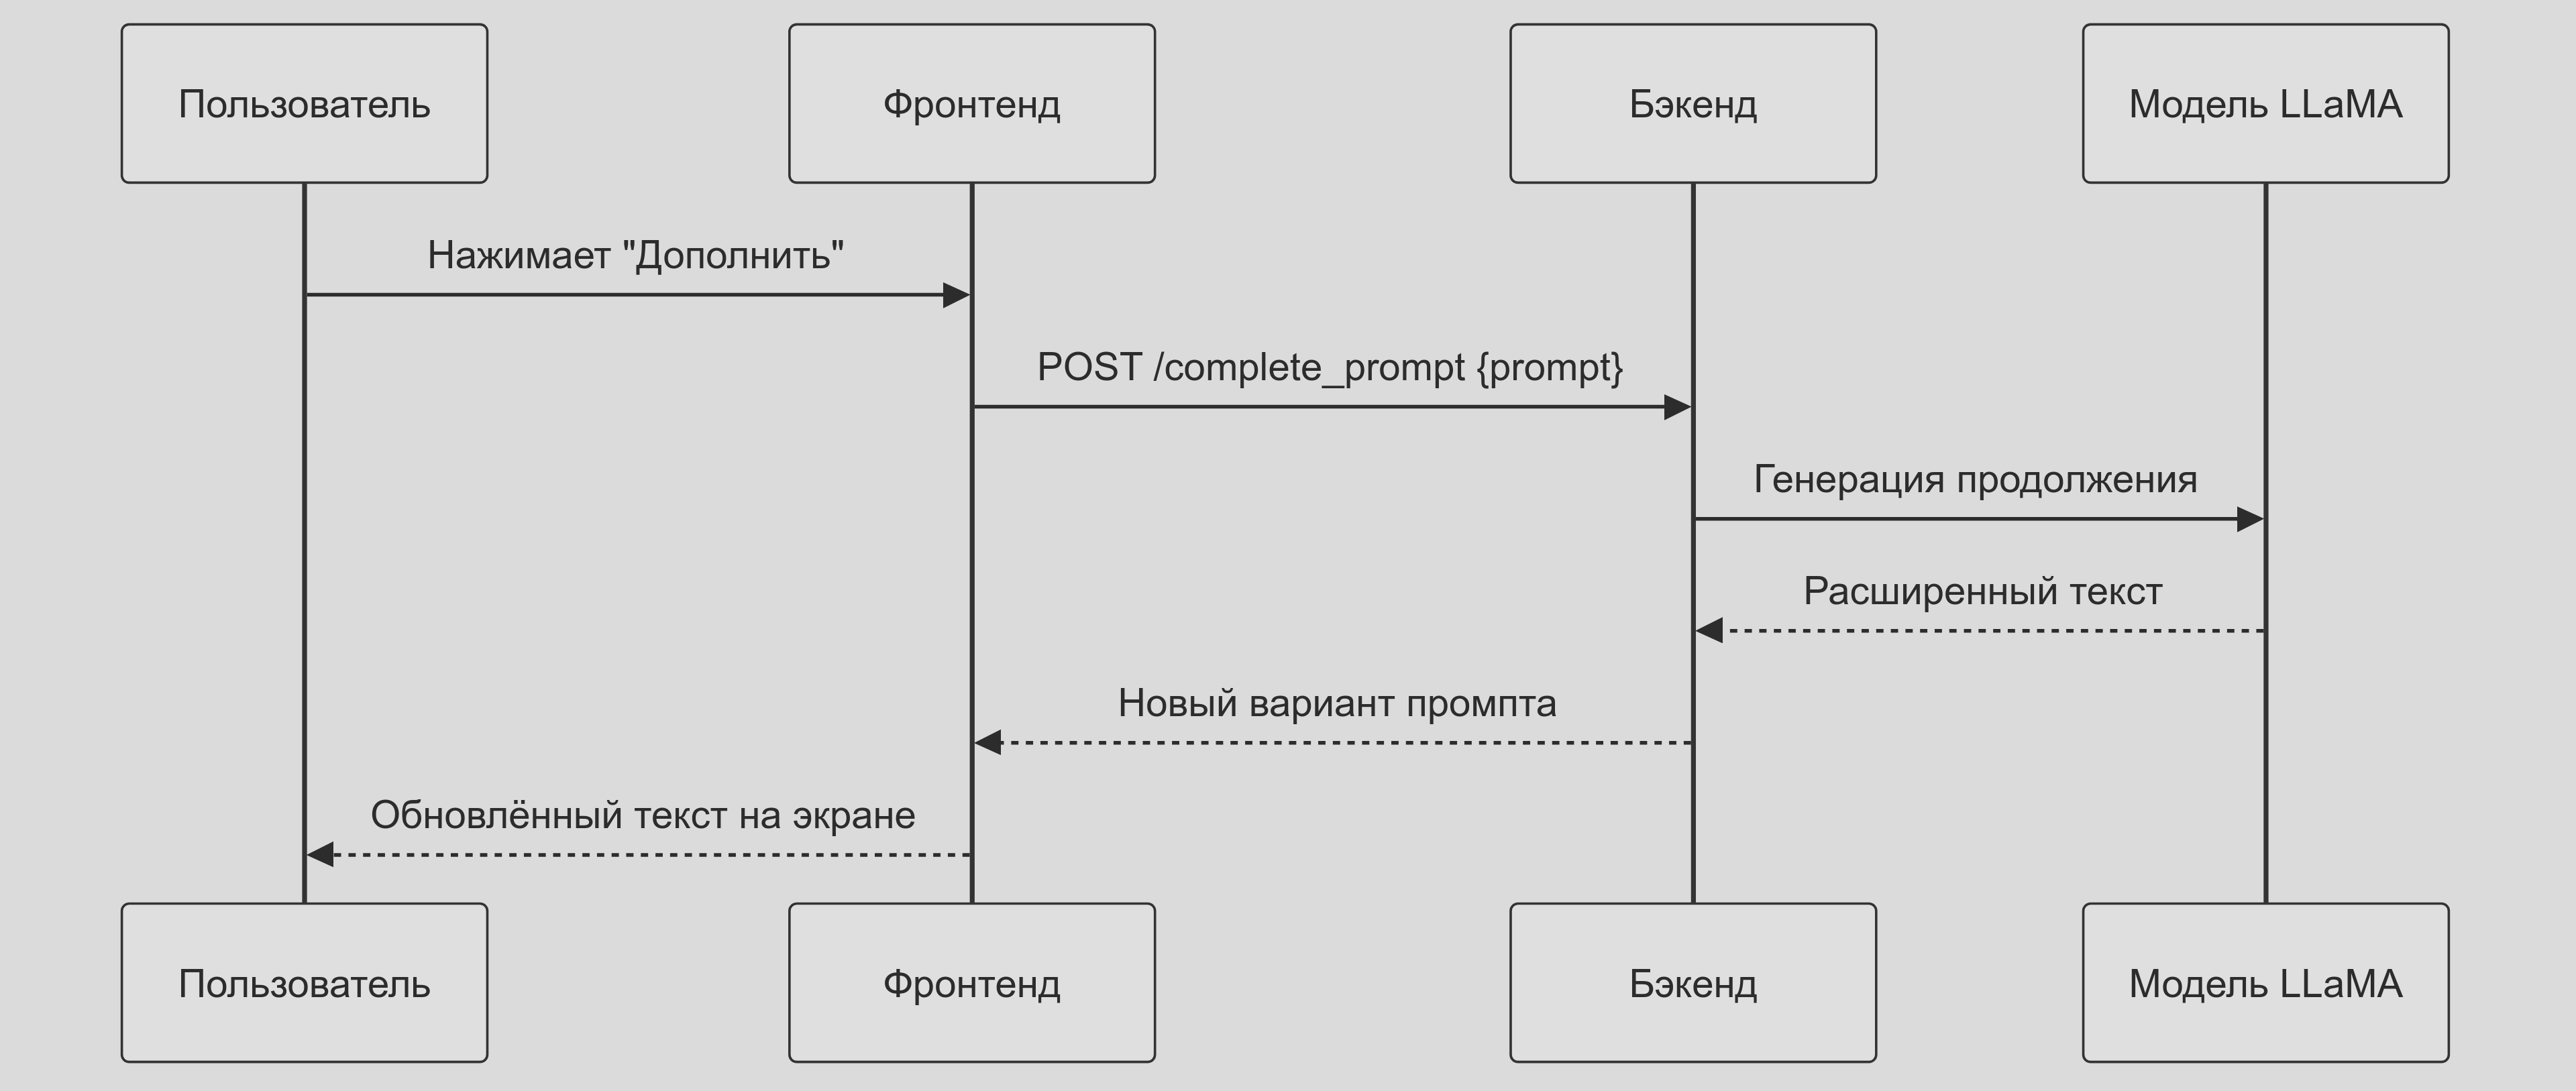
\includegraphics[width=1\textwidth]{picture/diploma-inter-algo-2.png}
    \caption{Алгоритм дополнения запроса}
    \label{algo-2}
\end{figure}
Дополнение запроса детализацией. Данная функция опирается на алгоритмы генерации текста с помощью модели LLaMA 8B. При нажатии пользователем кнопки «Дополнить» фронтенд отправляет текущий текст промпта на сервер (эндпойнт /complete prompt). Сервер вызывает специальную функцию, которая обращается к загруженной модели LLaMA. Алгоритм представлен на диаграмме \ref{algo-2} и может быть описан следуюoей последовательностью:
\begin{enumerate}[label=\arabic*.]
    \item Клиент отправляет исходный текст на сервер.
    \item Сервер формирует входную подсказку (Prompt) для LLaMA, используя шаблон <<Расширь описание \dots>.
    \item Модель генерирует продолжение с учётом заданных параметров (длина, температура и пр.).
    \item Полученные фразы автоматически добавляются к исходному промпту.

\end{enumerate}

Алгоритмически, основная интеллектуальная работа здесь выполняется языковой моделью. Предусмотрены некоторые меры для улучшения результата: например, если модель начала повторять исходный текст или уводит в сторону, сервер может отсечь первые токены генерации до появления новых данных. Также при реализации данного алгоритма используется специальное программное обеспечение – библиотека Hugging Face Transformers (или аналог) для работы с моделью. Поскольку LLaMA 8B не предоставляется готовым REST API, она интегрирована напрямую. PyTorch обеспечивает необходимый функционал генерации на GPU. Таким образом, алгоритм дополнения промпта сводится к задаче последовательного генерирования текста нейросетью – типичная задача, для которой используются наработки и функции библиотек машинного обучения.

Оценка качества промпта. Алгоритм оценки – это комбинация эвристических правил и, потенциально, моделей машинного обучения. В рамках данного проекта реализуется более простой, объяснимый подход на основе метрик текста. При вызове функции оценки (пользователь нажимает, либо автоматически при изменениях) фронтенд отправляет промпт на сервер (/evaluate prompt). Сервер вызывает функцию evaluate prompt(text), которая выполняет следующие шаги:
\begin{enumerate}[label=\arabic*.]
    \item Анализ длины и полноты. Вычисляется длина текста (в словах или символах). Если длина меньше некоторого порога (например, менее 3–5 слов), выставляется низкий базовый балл (такие запросы, как правило, слишком общие). Оптимальный диапазон длины – эмпирически, скажем, 10–20 слов для текстовых моделей, 5–15 слов для графических (со стилевыми тегами). Если запрос очень длинный (более 50–100 слов), тоже может снижаться балл – за избыточность.
    \item Проверка специфичности. Алгоритм может содержать список «пустых» слов (типа «изобрази», «сделай» – паразитные для промпта генерации изображения) и, наоборот, проверить наличие содержательных прилагательных, уточняющих фраз. Например, наличие хотя бы одного прилагательного или определяющего оборота может добавлять балл, так как уточняет запрос. В руководствах по промптингу подчёркивается, что специфичность и контекст повышают качество результата\cite{promptingguide:basics}. Следовательно, если промпт содержит детали (например, указание стиля, времени суток, эмоций персонажа и т.п.), это положительно влияет на оценку.
    \item Ясность формулировки. Проверяется, нет ли в тексте двусмысленностей или нерелевантных фрагментов. Этот пункт сложнее формализовать, но можно частично оценить по структуре предложения: если промпт состоит из нескольких несвязанных предложений или вопросительных форм (которые могут сбить модель), балл снижается. Например, запрос вида: «Нарисуй кота. Может дерево? Нет, лучше солнце.» явно плох по структуре – алгоритм может обнаружить наличие нескольких предложений или вопросительных знаков и снизить оценку.
    \item Учет модели. Если уже выбрана целевая модель, алгоритм может использовать разные профили оценки. Например, для изображения ценятся указания на визуальный стиль (реалистичный, мультяшный, 3D-рендер и т.д.) – их наличие повышает балл. Для текста ценится чётко поставленный вопрос или задача – наличие вопросительного знака при обращении к чат-боту, наоборот, может быть положительным (для диалоговой модели).
    \item Формирование итогового балла. Балл вычисляется на основании нескольких компонент. Например: score = length score + specificity score + clarity score + model adaptation score. Каждая в диапазоне 0–25, суммируя до 100. Данный подход позволяет объяснить оценку: «Ваш промпт слишком короткий, добавьте деталей» – если низкий length score, «промпт содержит противоречивые указания» – если clarity score низкий, и т.п. (В перспективе, можно подключить и саму LLaMA для оценки – например, попросив её оценить промпт по шкале, но это менее детерминированно.)
    \item Возврат балла. Сервер возвращает число от 0 до 100. Клиент отображает его, при этом возможно сопроводить коротким вердиктом (например, «Среднее качество» при 50–70, «Отличный промпт» при >80).
\end{enumerate}
Этот алгоритм легко модифицировать под новые критерии, его можно обучить (если бы были данные промптов с оценками, можно настроить веса правил или модель классификатор). Пока же он реализован на основе здравого смысла и рекомендаций по написанию промптов\cite{vc:prompt}, \cite{promptingguide:basics}. Программно реализация выполнена на Python: для лингвистического анализа можно использовать стандартные библиотеки (например, NLTK или simple pos-tagging для выделения частей речи, если нужно искать прилагательные). Однако в простейшем варианте достаточно операций над строками, что не требует внешних зависимостей. Важно отметить, что время выполнения этого алгоритма невелико – порядка нескольких миллисекунд, т.к. текст анализируется без тяжёлых моделей. Поэтому оценка может обновляться практически мгновенно при каждом изменении запроса.

Реструктуризация промпта под модель. Алгоритм реструктуризации заключается в применении определённого набора правил трансформации текста в зависимости от целевой модели. Эти правила основаны на известных требованиях/особенностях промптов для разных генераторов. Реализация может быть как шаблонной (набор if/else в коде), так и с участием нейросети (например, снова задействовать LLaMA: «Переформулируй запрос для такой-то модели»). В первом прототипе достаточно правила:
\begin{enumerate}[label=\arabic*.]
    \item Для модели изображения (Fusion Brain/Kandinsky):\begin{enumerate}[label=1.\arabic*.]
        \item Удалить обращение к модели в повелительном наклонении. Например, фразы вроде «нарисуй», «сгенерируй картинку:» не несут содержания для модели, их следует убрать.
        \item Выделить негативные указания. Если в тексте есть конструкции «не используй ...», «без ...», они преобразуются в отдельный негативный промпт (для Kandinsky предусмотрено поле negativePromptUnclip). Алгоритм: найти ключевые слова «не», «без», собрать последующие слова до запятой или конца – это будет отрицательный промпт.
        \item Проверить язык описания. Kandinsky 3.1 понимает и русский, и английский\cite{fusionbrain:docs}. Здесь не нужно перевода, но важно убедиться, что промпт цельный на одном языке (смешение языков нежелательно).
        \item Возможно, добавить стандартные атрибуты, если их нет: например, многие художники добавляют стилистические теги («арт», «реалистично», «аниме-стиль»). Если пользователь ничего про стиль не указал, алгоритм мог бы по умолчанию добавить что-то нейтральное (но чаще стиль лучше оставить пустым – Fusion Brain и так принимает параметр style, который по умолчанию = NONE).
        \item Итогом алгоритма станет либо изменённая строка промпта (если мы решим не разделять, а просто убрать лишние слова), либо структура с полями: main\_prompt и negative\_prompt. Сервер знает, что для FusionBrain надо использовать оба. На стороне клиента это может отобразиться или остаться скрытым – по решению.
    \end{enumerate}
    \item Для языковой модели (LLaMA или подобные): 
    \begin{enumerate}[label=2.\arabic*.]
        \item Если исходный промпт больше походил на описание картинки (например, перечисление объектов без вопроса), а цель – текст, возможно, стоит преобразовать его в форму задания или вопроса. Например, промпт «кот сидит на дереве ночью» для чат-бота LLM непонятен – алгоритм мог бы добавить «Опиши сцену: кот сидит на дереве ночью.» либо обернуть это в вопрос: «Что произошло: кот сидит на дереве ночью? Расскажи историю.» Но такие преобразования могут оказаться слишком творческими. Вероятно, лучше минимально менять текст.
        \item Удалить специфические теги или слова, характерные для графических запросов (типа «4K», «highly detailed») – в текстовой модели они бессмысленны.
        \item Если целевая языковая модель – диалоговая, можно добавить, например, пометку «User: \{prompt\} Assistant:» для внутренних нужд (в LLaMA 2 есть формат входа с метками ролей).
    \end{enumerate}
\end{enumerate}
В целом алгоритм реструктуризации во многом состоит из поиска и замены. Он оперирует строкой: ищет определённые шаблоны (регулярные выражения или ключевые фразы) и преобразует их. Его сложность невысока, реализация на Python с библиотекой re или просто методами строк. При расширении на новые модели (например, аудиогенерация) нужно будет добавить соответствующие правила (например, убрать слова «изображение», заменить их на «звук», и т.д.).

Предварительный просмотр результата представлен, как последовательность показанную на диаграмме \ref{algo-3}
\begin{figure}[htbp]
    \centering
    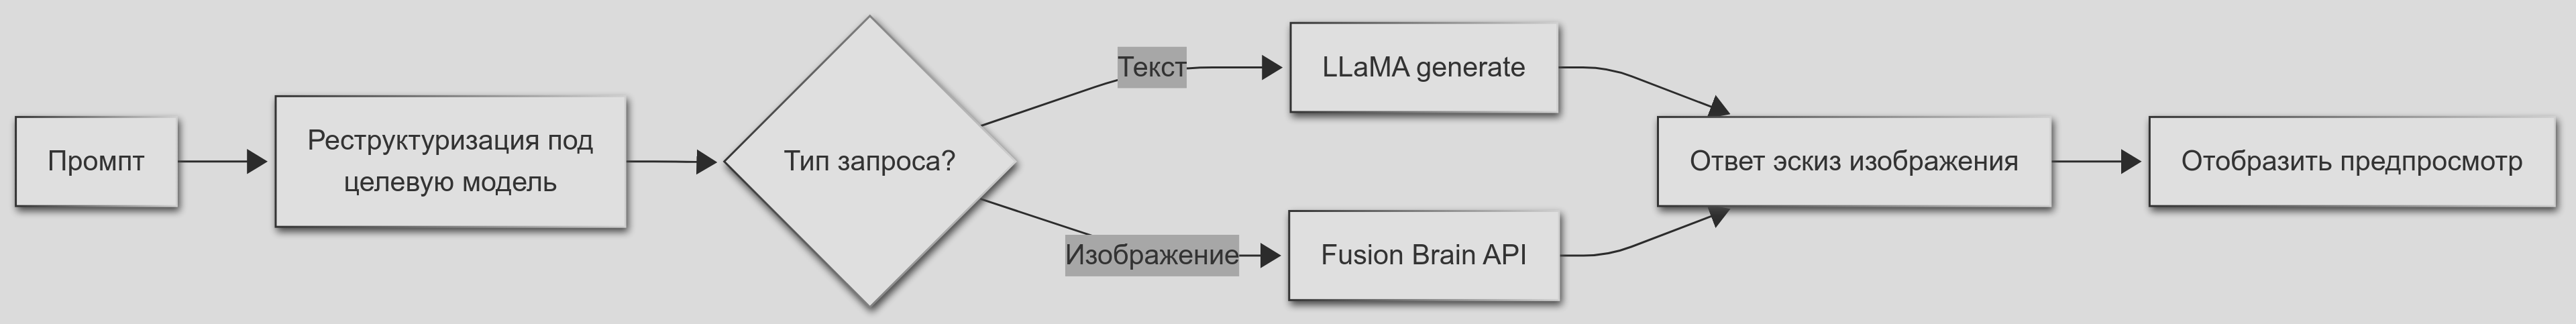
\includegraphics[width=1\textwidth]{picture/diploma-inter-algo-3.png}
    \caption{Алгори предпросмотра  результата запроса}
    \label{algo-3}
\end{figure}


Данная последовательность заключается в седующих шагах:
\begin{enumerate}[label=\arabic*)]
    \item Пользователь нажимает кнопку «Предпросмотр».
    \item Фронтенд отправляет запрос \texttt{/preview} с текстом и типом результата (текст/изображение).
    \item Бэкенд корректирует промпт и определяет модель – LLaMA или Fusion Brain.
    \item Для текста генерируется ответ, для изображения – вызов API Kandinsky.
    \item Полученные данные сервер возвращает в JSON или base64, затем фронтенд отображает предварительный результат.
    \item Пользователь может повторить предпросмотр, внося корректировки в промпт.
\end{enumerate}

Таким образом, набор описанных алгоритмов (редактирование, дополнение, оценка, реструктуризация, предпросмотр) в сочетании с перечисленными фреймворками и библиотеками обеспечивает требуемый функционал платформы.

\subsection{Конструктивно-технологические решения}
Разработка программного обеспечения всегда сопряжена с выбором не только алгоритмов, но и конкретных технологий, а также способов их интеграции и развертывания. В данном разделе рассматриваются решения, касающиеся архитектуры системы в техническом (конструктивном) плане и организационно-технологические аспекты: структура развёртывания компонентов, способ обеспечения их совместной работы, обоснование выбранных технологий с точки зрения инфраструктуры и будущей поддержки.

\par Логическая и физическая структура системы. Платформа разделена на несколько компонентов, как описано в архитектуре: фронтенд (Vue.js), сервер (FastAPI + модели) и база данных (PostgreSQL). Логически они взаимодействуют через чёткие интерфейсы (HTTP API, SQL). Физически для упрощения развертывания на практике они могут быть размещены на одном сервере или виртуальной машине, либо на нескольких, в зависимости от требований к производительности.
Для целей дипломного проекта предполагается локальное развертывание: на одной машине запускаются все нужные сервисы. Это упрощает демонстрацию и тестирование.

Использование контейнерных технологий. Для облегчения установки и переноса системы был выбран подход с применением Docker-контейнеров.
Контейнеризация обеспечивает единообразие среды (исключает проблему «у меня работает, у вас нет»), а также облегчает деплоймент на сервер. Компоненты запускаются оркестратором (например, Docker Compose прописывает три сервиса: web, api, db, и нужные сети между ними).

Выбор технологий и обоснование. Принятые технологические решения обусловлены требованиями к функционалу и ограничениями ресурсов:
FastAPI vs альтернативы: рассматривались Flask и Django. Flask слишком низкоуровневый и требует больше ручной работы по структуре проекта и валидации данных. Django избыточен (целый MVC-фреймворк) для задачи создания API. FastAPI же специально создан для API, поддерживает асинхронность и даёт высокую производительность на уровне, близком к Node.js или Go благодаря использованию Uvicorn/Starlette\cite{easyoffer:fastapi}. Кроме того, его встроенные механизмы (взаимодействие с Pydantic) упрощают безопасную обработку входных данных (что хорошо для безопасности – см. раздел 9) и автоматическое документирование. Достоинства FastAPI – высокая производительность и простота – стали решающими факторами\cite{fastapi:practicum}.

PyTorch (LLaMA) vs внешние API: Одним из ключевых решений было использовать локальную модель LLaMA 8B вместо обращения к, например, OpenAI API для текстовых генераций. Во-первых, это обеспечивает автономность – система может работать полностью офлайн (что актуально, если данные пользователей конфиденциальны и их нельзя отправлять во внешние сервисы). Во-вторых, локальная модель позволяет настроить работу так, как нужно (например, ограничить длину ответа, получить скрытые состояния, если требуется). И хотя качество LLaMA 8B может быть ниже GPT-3.5, для целей предпросмотра и оценки промптов она справляется (тем более, что она из семейства моделей Meta, известных хорошим качеством при оптимальном количестве параметров)\cite{llama:wiki}. Это решение потребовало наличия GPU, но в разделе 8 обосновываются необходимые аппаратные ресурсы – они достижимы. Кроме того, открытость кода LLaMA позволяет при необходимости тонко донастроить модель на специфичные данные (в будущем, например, можно обучить её лучше оценивать промпты).

Fusion Brain API vs локальная генерация изображений: Для генерации изображений был выбран готовый API (Fusion Brain, предоставляющий доступ к модели Kandinsky 3.1)\cite{sitelabs:kandinsky}. Альтернативой могло быть поднятие локального сервиса Stable Diffusion или самой модели Kandinsky. Однако это потребовало бы дополнительных больших вычислительных ресурсов (еще один крупный вес модели, отдельный GPU). С учётом ограничений оборудования и времени, было рациональнее воспользоваться внешним сервисом. Fusion Brain выбран, так как это российская платформа, свободно доступная для использования (модель Kandinsky бесплатна и поддерживает русский язык\cite{sitelabs:kandinsky}), что соответствует целевой аудитории. Также, Kandinsky 3.1 – одна из самых продвинутых моделей генерации изображений на момент разработки, демонстрирует высокое качество (почти на уровне MidJourney в ряде случаев). Использование её API позволяет пользователям получать высококачественные превью изображений без необходимости самим иметь мощный GPU. Таким образом, это решение – компромисс между качеством и сложностью: перенести нагрузку по генерации изображений на удалённый сервис. Конечно, от сервиса требуется интернет-соединение, но в современных условиях это приемлемо.Vue.js vs React/Angular: Для фронтенда выбрана Vue.js из-за её более низкого порога вхождения и удобства для постепенного внедрения. Разработчики, особенно знакомые с HTML/CSS, обычно легче осваивают Vue, тогда как React требует писать больше шаблонного кода, а Angular – слишком громоздок для небольшого проекта. Vue известен своей доступностью и отличной документацией\cite{vuejs:wiki}. Кроме того, Vue прекрасно подходит для реализации drag-and-drop интерфейсов, существующие плагины и сообщество упрощают эту задачу. В итоге, Vue.js обеспечивает быструю разработку интерактивного интерфейса при небольших затратах времени.PostgreSQL vs SQLite/Другие СУБД: Для хранения данных выбрана PostgreSQL, хотя объем сохраняемой информации невелик. Обоснование – промышленная надежность и масштабируемость. PostgreSQL – открытая ORDBMS с более чем 30-летней историей разработки, одна из самых продвинутых БД с открытым кодом\cite{postgresql:skillfactory}, поддерживающая строгие гарантии сохранности данных. В случае расширения проекта (например, ведение большой базы промптов, статистики) PostgreSQL справится без проблем. Кроме того, использовать ее удобно в Docker-контейнере, а также многие ORM поддерживают ее «из коробки». SQLite могла бы быть проще на этапе прототипа, но для веб-приложения с потенциально несколькими пользователями параллельно SQLite не так надёжен (он однопоточный). Поэтому предпочтение отдано PostgreSQL – надежность данных и возможность роста.Организация разработки и деплоймента. При реализации данного проекта был использован подход непрерывной интеграции: код хранится в системе контроля версий (Git), настроено автоматическое построение Docker-образов при обновлении. Это облегчает тестирование на разных машинах (можно быстро развернуть весь стек с помощью docker-compose up). Также применялись практики разбиения задач: UI и backend разрабатывались отдельно, через согласованный API (для проверки использовались инструменты типа Swagger UI, сгенерированный FastAPI автоматически, что помогало фронтенд-разработчику видеть, какие запросы доступны).

Безотказность и отказоустойчивость. Конструктивно, система спроектирована с учетом потенциальных отказов. Если падает внешний сервис (Fusion Brain), платформа всё ещё функционирует частично (редактирование, оценка, даже текстовое preview через LLaMA продолжает работать). Пользователю выдаётся сообщение об ошибке внешнего сервиса, но само приложение не «рушится».Если по какой-то причине недоступна модель LLaMA (например, не хватило памяти и процесс упал), FastAPI возвращает код ошибки при попытке её использовать, а интерфейс может предупредить, что текстовый preview временно недоступен. При этом другие функции (хранение истории, редактирование) работают.База данных – единая точка хранения. В случае сбоя БД (например, отключилась) сервер не сможет записать/прочитать историю или выполнить логин. Такие ситуации обрабатываются: сервер выдаст ошибку 500, а на UI можно отобразить уведомление «Сервис временно недоступен». Чтобы повысить надежность, в продуктивной эксплуатации СУБД обычно запускают с механизмами репликации, регулярного бэкапа. Для дипломного прототипа достаточно периодически сохранять дамп БД и, при необходимости, перезапустить контейнер БД (данные не потеряются благодаря использованию volume для хранения файлов БД на хосте).

В итоге, принятые конструктивно-технологические решения – использование контейнеризации, разделение на компоненты, выбор оптимального стека – обеспечили надежную и гибкую основу для реализации платформы. Этот подход облегчает как текущую разработку (каждый компонент можно развернуть и отладить независимо), так и дальнейшее сопровождение (обновление отдельного сервиса не нарушит работу остальных при соблюдении контракта API). Все решения согласованы с требованиями: например, необходимость GPU для LLaMA связана с требованием локальной генерации текста, а привлечение Fusion Brain – с требованием высококачественного preview изображений. Такое сочетание решений подтверждает целесообразность и реализуемость проекта в заданных условиях.

\subsection{Безопасность и аутентификация}

При проектировании платформы уделяется серьёзное внимание вопросам безопасности – как защите данных пользователей, так и устойчивости системы к злонамеренным воздействиям. Также реализованы механизмы аутентификации, гарантирующие доступ к функционалу только авторизованным лицам (в рамках данного проекта – зарегистрированным пользователям с ролью разработчика/художника). Ниже описаны меры, принятые для обеспечения безопасности и процессы аутентификации пользователей.


\begin{figure}[htbp]
\centering
    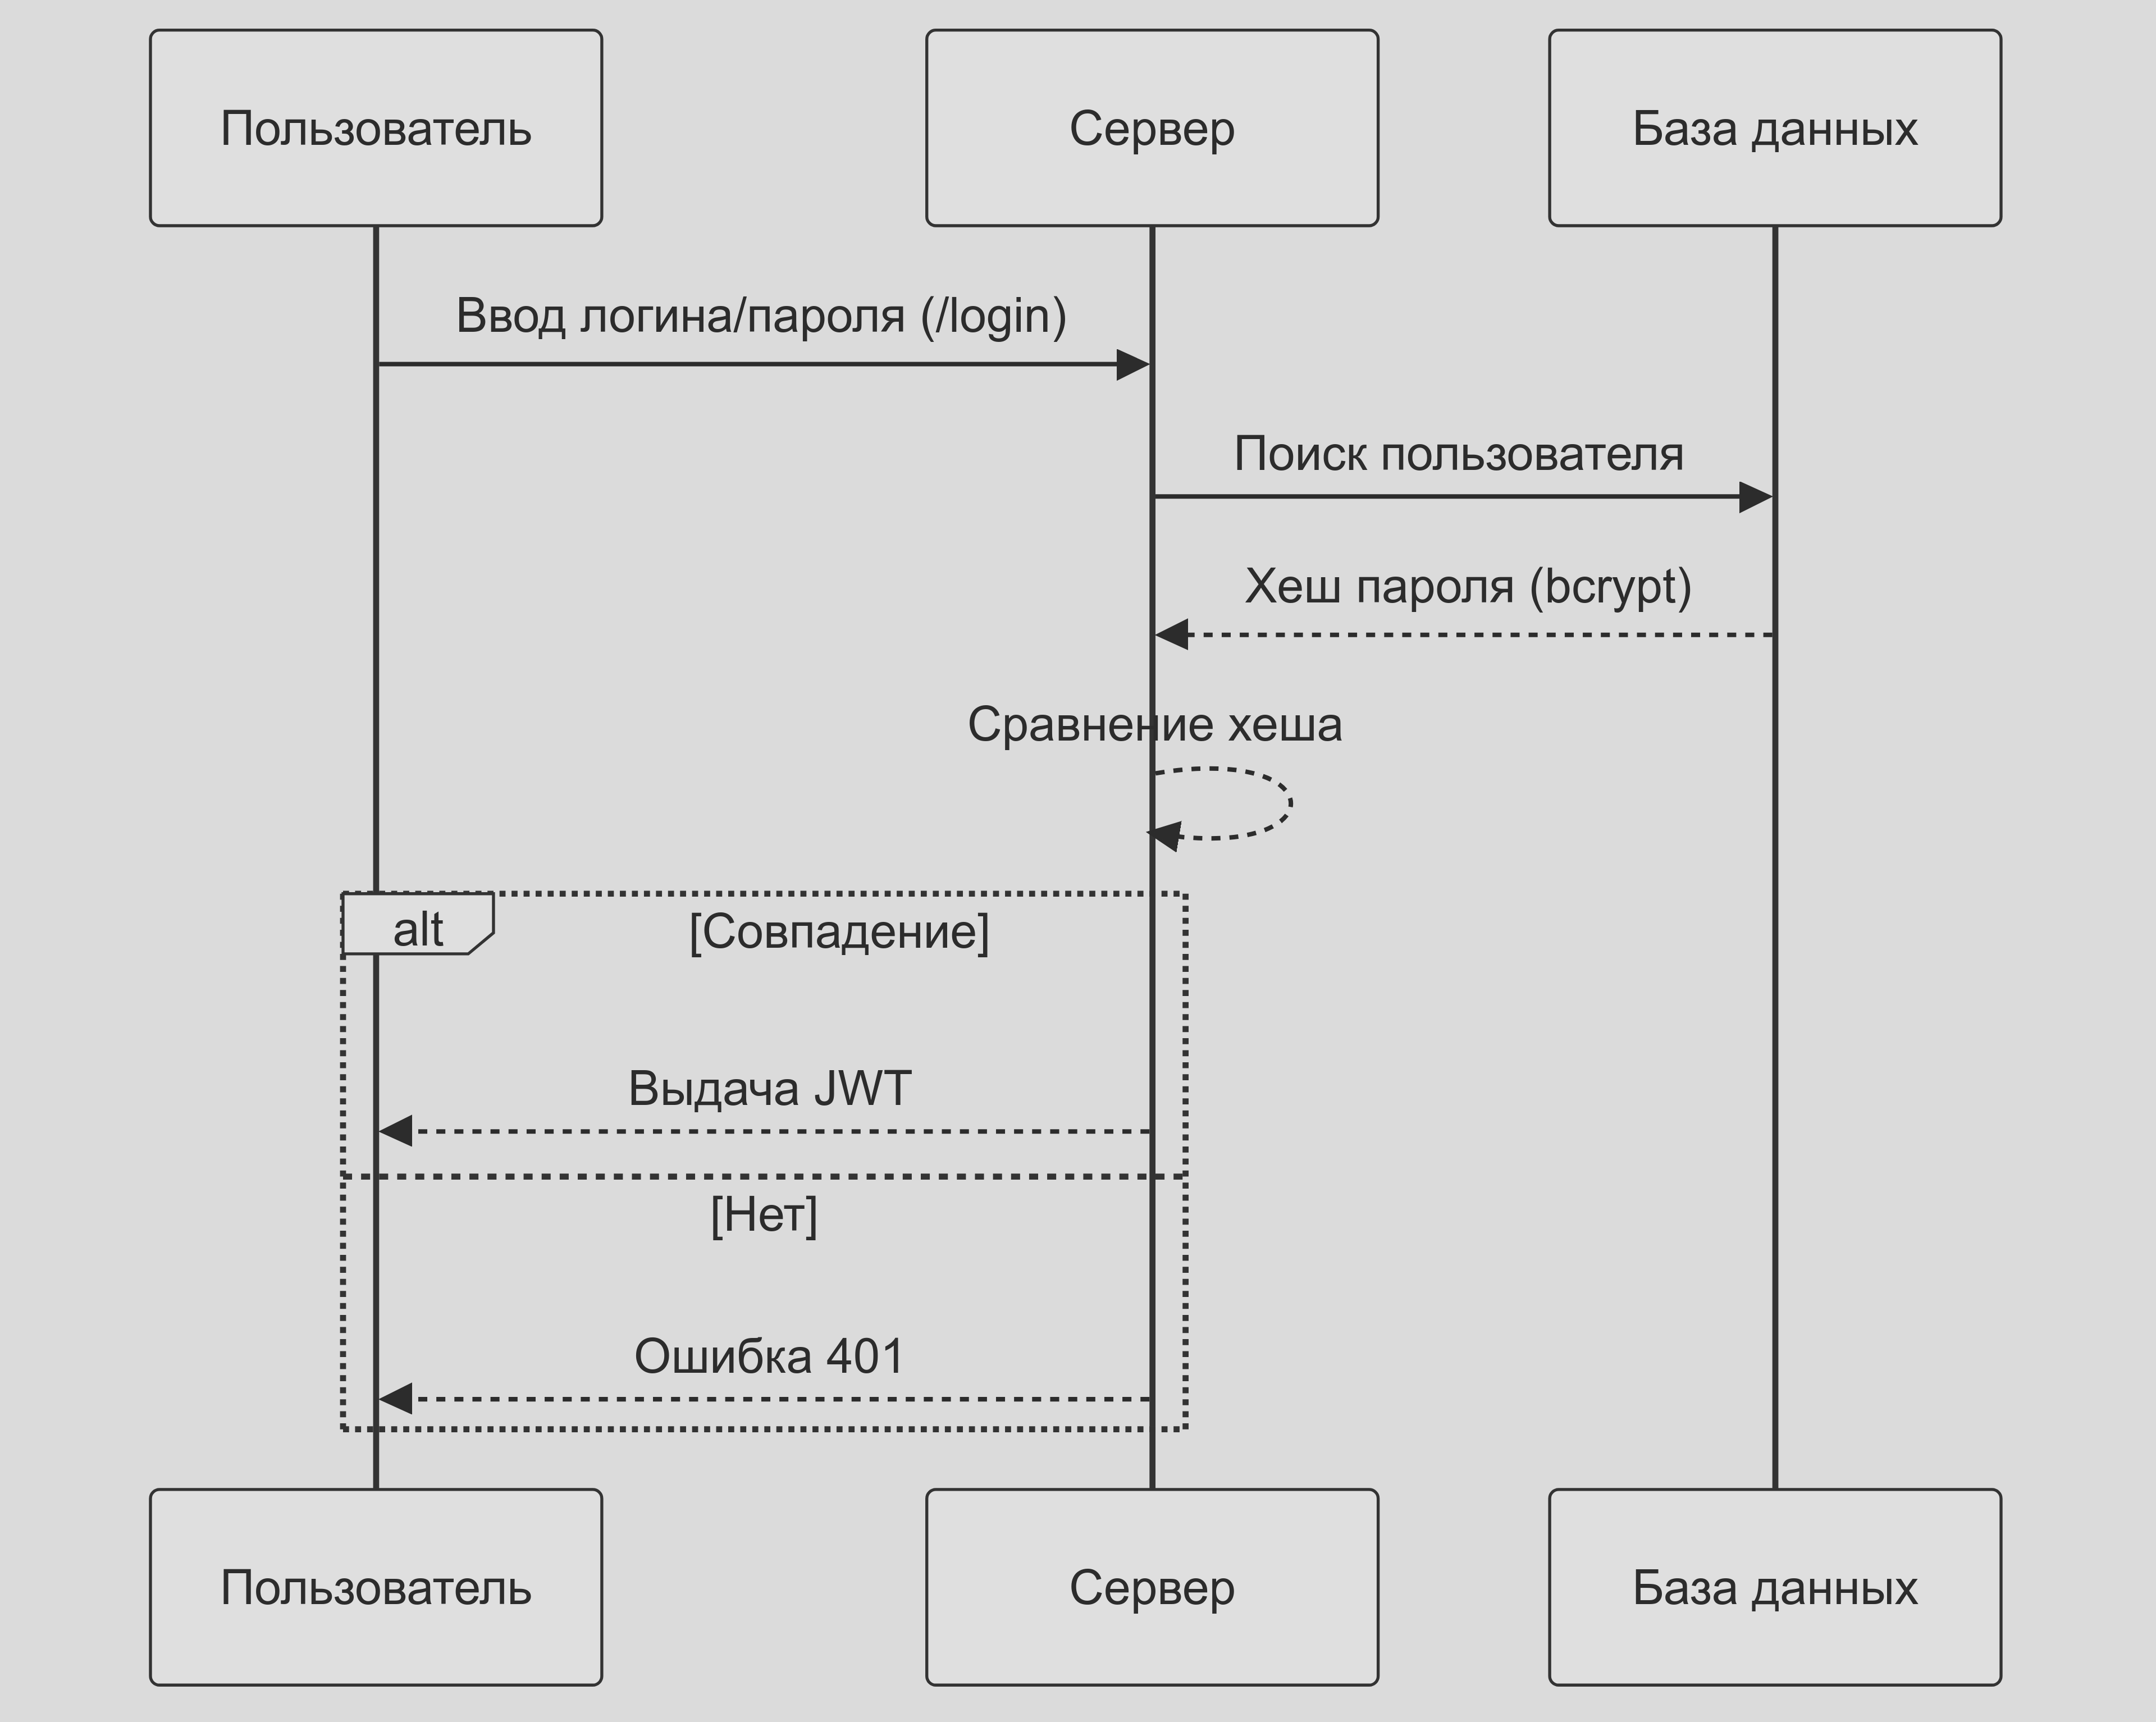
\includegraphics[width=1\textwidth]{picture/diploma-deffence-algo-1.png}
\caption{Схема аутентификации пользователя}
\label{diagram_auth}
\end{figure}


Платформа использует систему учётных записей с безопасным хранением паролей (bcrypt) и выдачей JWT-токенов. Все запросы к защищённым эндпойнтам требуют валидного JWT, что гарантирует доступ только авторизованным пользователям. Общая схема аутентификации показана на рис.~\ref{diagram_auth}.


\begin{figure}[htbp]
\centering
    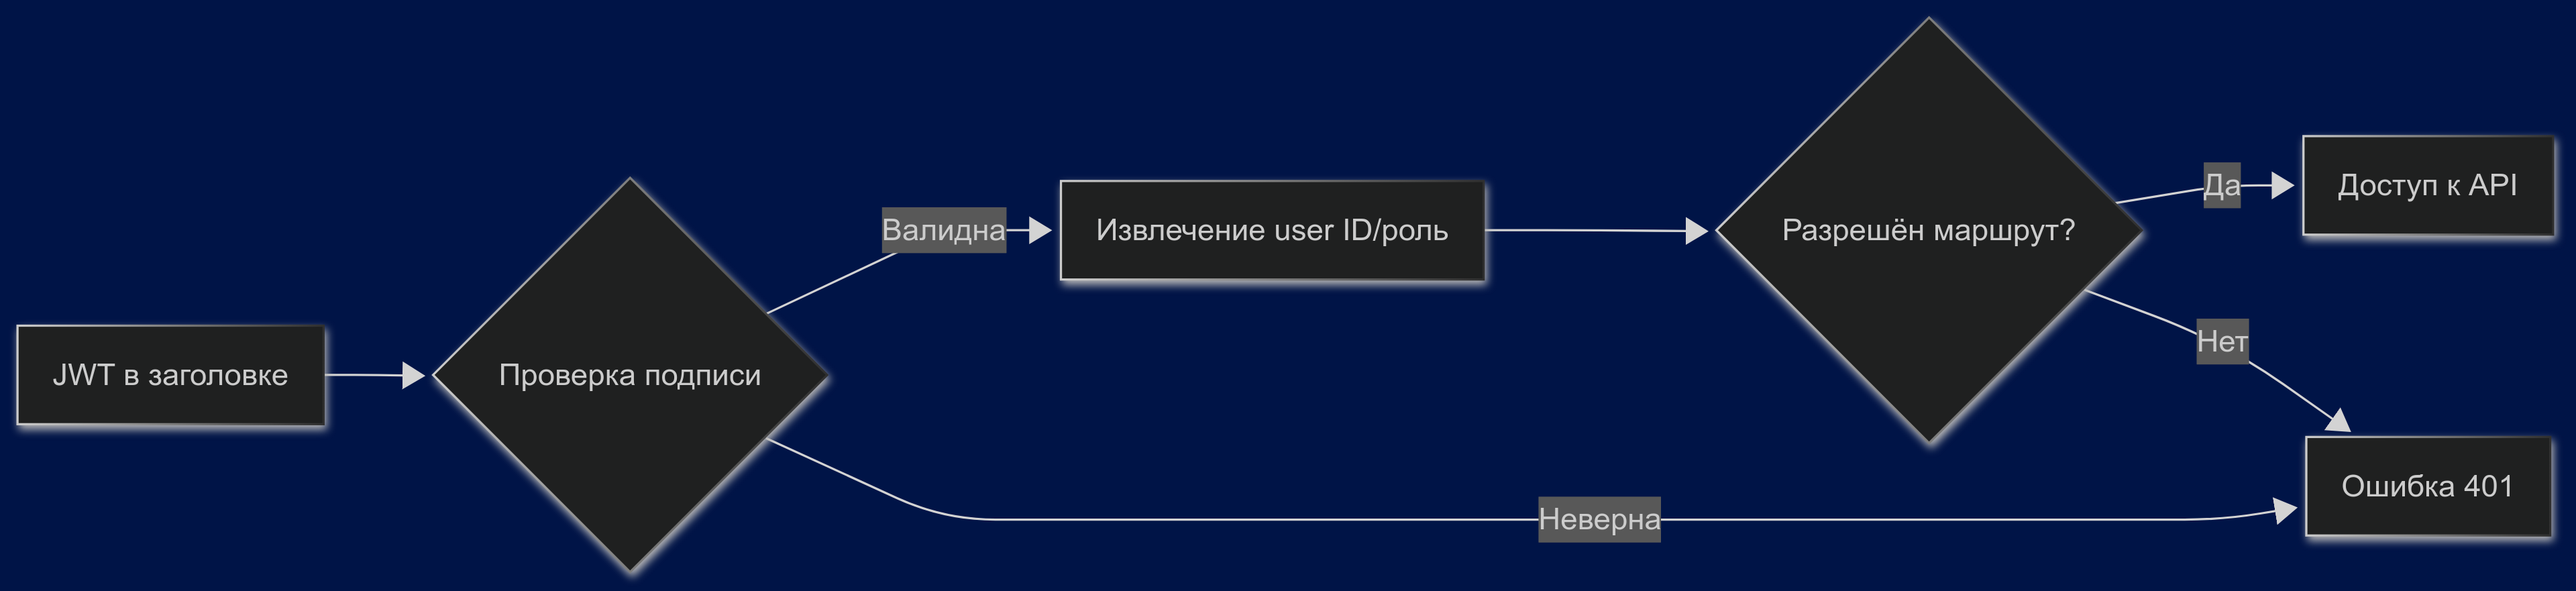
\includegraphics[width=1\textwidth]{picture/diploma-deffence-algo-2.png}
\caption{Проверка и использование JWT-токена}
\label{diagram_jwt}
\end{figure}

Разграничение доступа. На данный момент все аутентифицированные пользователи имеют одинаковые права (могут редактировать свои промпты, получать preview и т.д.). Однако система спроектирована с возможностью введения ролей. Например, можно добавить роль администратор, которому доступны дополнительные сведения (просмотр истории всех пользователей, управление учётными записями).  JWT содержит зашифрованные данные (id, роль), подписанные секретным ключом. При каждом запросе на сервер фронтенд прикрепляет токен в заголовке \texttt{Authorization}. Сервер валидацией подписи убеждается, что пользователь активен, и пускает к ресурсам согласно роли (рис.~\ref{diagram_jwt}).

Передача данных по сети. Взаимодействие клиент-сервер происходит по HTTP(S). Для безопасности в рабочей эксплуатации необходимо использовать протокол HTTPS с валидным SSL-сертификатом. Это гарантирует шифрование всего трафика: логинов, паролей, токенов, а также передаваемых промптов и сгенерированных результатов. Настройка HTTPS достигается либо за счёт reverse-proxy (например, Nginx с SSL передаёт на Uvicorn), либо используя встроенные возможности UVicorn + Hypercorn. Шифрование критически важно, чтобы злоумышленник в одной сети с пользователем не смог перехватить JWT-токен или крадущим образом прочесть содержимое передаваемых промптов.

Защита API и данных. Внутри серверного кода внедрены следующие меры безопасности:
\begin{enumerate}[label=\arabic*.]
    \item Шифрование (HTTPS) защищает логины, пароли и промпты.
    \item Валидация данных (Pydantic) и ORM предотвращают SQL-инъекции.
    \item Ключи и конфигурация (например, API-ключи) хранятся только на сервере.
    \item Длина промпта ограничена (до 1000 символов), чтобы избежать злоупотреблений.
    \item История запросов и конфиденциальные данные изолированы по user\_id.
\end{enumerate}

Защита данных пользователя. Помимо паролей, которые хранятся в виде хешей, следует отметить и защиту содержимого истории промптов. Хотя они не столь конфиденциальны, все же это интеллектуальная собственность пользователя (особенно для художника: удачно сформулированный промпт – ценность). Поэтому история запросов каждого пользователя закрыта от других (как описано), а также от постороннего доступа извне (невозможно без JWT вытащить эти данные через API). При хранении на диске бэкапы БД также должны быть защищены (например, шифрованы или доступны только администратору).

Безопасность модели LLaMA. Локальная модель – это код, который мы запускаем. Он загружен из надежного источника (предполагается официальные веса). Тем не менее, есть аспект: промпт, подаваемый в модель, может быть сконструирован злоумышленником так, чтобы использовать уязвимости модели. Например, prompt injection – когда пользователь даёт особый запрос, заставляющий модель игнорировать инструкции и, предположим, выдать скрытую информацию или выполнить чужой код. В нашем случае LLaMA 8B – модель генерации текста, она не выполняет произвольный код, потому тут скорее вопрос нежелательного контента. Если дать ей оскорбительный или опасный запрос, она может сгенерировать нежелательный текст. Чтобы это смягчить, можно внедрить фильтр контента на выходе модели (например, использовать модель-модератор или простой список стоп-слов для выходного текста). Так, если LLaMA вдруг выдаст что-то, нарушающее правила (нецензурную брань, персональные данные), платформе следовало бы отфильтровать. В контексте дипломного прототипа это тонкость, но для полноты стоит упомянуть: Fusion Brain (Kandinsky) имеет встроенный контент-фильтр на сервере (он не создаст запрещенные изображения, а вернёт заглушку).Для LLaMA можно использовать open-source модель модератора или хотя бы явно не разрешать некоторые запросы (но мы предполагаем, что наши пользователи – благонадежные разработчики/художники).Обновления безопасности. Регулярно обновляется программное обеспечение: библиотеки (FastAPI, PyTorch) – это важно, так как в них могут обнаруживаться уязвимости. Использование контейнеров позволяет легко обновлять среду (например, переходить на новые образы с обновлениями безопасности OS). Также внутренний секретный ключ для JWT хранится в .env, его необходимо генерировать длинным и случайным, и при подозрении на утечку менять (это обеззопасит прошлые токены, которые станут недействительными).

Безопасность инфраструктуры. Сервер, на котором размещается система, должен быть защищен: настроен файрвол (открыты только необходимые порты – 443 для HTTPS, 80 может редиректиться на 443, и, возможно, 22 для SSH админа). Доступ к серверу по SSH – только администратору с ключом, либо через VPN. PostgreSQL сервер, если отдельный, то либо локальный, либо за firewall – не в открытом интернет (или по крайней мере с ограничением по IP доступа до сервера приложения). Резервные копии БД следует хранить шифрованно, если хранятся вне сервера.

Подытоживая: аутентификация в системе реализована посредством логина/пароля с безопасным хранением (bcrypt-хеши) и выдачей JWT-токенов. Авторизация (проверка прав) – все основные маршруты требуют валидного токена, и пользователь имеет доступ только к своим данным. Безопасность данных и кодов обеспечивается на нескольких уровнях: шифрование канала (HTTPS), валидация входа, защита БД от инъекций, ограничение привилегий. Принятые меры соответствуют общепринятым практикам веб-безопасности (OWASP) и учитывают особенности нашей платформы (включая интеграцию ML). Таким образом, система защищена от большинства распространённых угроз: утечки учётных данных, несанкционированного доступа к данным, перехвата трафика, SQL-инъекций, brute-force атак на пароли и др. Это создаёт прочную основу доверия для пользователей: они могут безопасно использовать платформу, не опасаясь за сохранность своих персональных данных и уникальных промптов.
\subsection{Вывод}
В разделе проектирования была разработана подробная архитектура и техническое решение для платформы интерактивного формирования, оценки и предварительного просмотра запросов (промптов) к языковым и генеративным нейросетям. Платформа построена по принципу клиент-сервер и включает серверное приложение на FastAPI, взаимодействующее с локальной LLM-моделью LLaMA 8B (PyTorch) и внешним API Fusion Brain (модель Kandinsky 3.1) для генерации изображений, веб-клиент на Vue.js для удобного интерфейса и базу данных PostgreSQL для хранения пользовательских данных.

На основании требований были спроектированы конкретные методики реализации всех заявленных функций: редактирование промптов как в текстовом режиме, так и путём перетаскивания токенов; автоматизированное дополнение описаний с использованием возможностей большой языковой модели; вычисление метрики качества промпта по набору правил; преобразование формата запросов под требования разных моделей; механизм preview, позволяющий быстро получать отклики от модели (текстовые – через LLaMA, графические – через FusionBrain) и показывать их пользователю. Каждый из этих функциональных блоков был рассмотрен с точки зрения алгоритмов и программных средств, что показало реализуемость поставленных задач.

Разработанная архитектура системы демонстрирует баланс между использованием локальных ресурсов и облачных сервисов: тяжёлая языковая модель размещена локально, что даёт независимость от внешних API и быстрый отклик, тогда как генерация изображений делегирована специализированному удалённому сервису для достижения высокого качества без чрезмерных требований к оборудованию. Клиентское приложение на Vue.js обеспечивает интерактивность и отзывчивый интерфейс, удовлетворяющий потребностям как технических, так и творческих пользователей.

В ходе проектирования были приняты обоснованные схемотехнические, алгоритмические, программные и конструктивно-технологические решения. Выбор FastAPI и PyTorch на сервере обеспечил высокую производительность и гибкость при интеграции ML-модели, выбор Vue.js на фронтенде – удобство реализации сложного UI. Внедрение JWT-аутентификации, bcrypt-хеширования паролей и других мер безопасности позволило создать надежный механизм защиты данных, что немаловажно для приложения, работающего с пользовательским контентом.

Проектирование учитывало профиль пользователей системы (разработчики и художники) – в решениях особое внимание уделено удобству интерфейса (двойной режим редактирования, визуальный просмотр результатов), а также обеспечению того, чтобы ни одна из групп не была технически ограничена в использовании платформы. Все требования заказчика по функционалу удовлетворены предлагаемым дизайном: система позволяет интерактивно экспериментировать с промптами, улучшать их качество и сразу видеть, к чему эти улучшения приводят, что в конечном итоге повышает эффективность работы с нейросетевыми моделями.

В заключение, спроектированная платформа представляет собой целостное решение, сочетающее современные веб-технологии и методы работы с нейросетями. Она обладает модульностью и расширяемостью – в будущем возможно подключение новых моделей (например, других языковых моделей или генератора музыки) или внедрение дополнительных функций (таких как библиотека шаблонов промптов, совместное редактирование и пр.) без пересмотра базовых принципов архитектуры. Проектировочные решения прошли проверку на соответствие требованиям: они реалистичны и подтверждены ссылками на технические характеристики используемых компонентов.
Разработка данной системы внесет вклад в сферу prompt engineering, предоставив специалистам удобный инструмент для отладки запросов. Проектирование завершено, и следующим этапом является непосредственная реализация (кодирование) согласно изложенному дизайну, после чего платформу предстоит протестировать в условиях, приближенных к боевым, чтобы убедиться в выполнении всех требований и высоком качестве полученного решения.